
\documentclass[DIV=calc, paper=a4, fontsize=11pt, twocolumn, spanish]{scrartcl}	 % A4 paper and 11pt font size

\usepackage{lipsum} % Used for inserting dummy 'Lorem ipsum' text into the template
\usepackage[protrusion=true,expansion=true]{microtype} % Better typography
\usepackage{amsmath,amsfonts,amsthm} % Math packages
\usepackage[svgnames]{xcolor} % Enabling colors by their 'svgnames'
\usepackage[hang, small,labelfont=bf,up,textfont=it,up]{caption} % Custom captions under/above floats in tables or figures
\usepackage{booktabs} % Horizontal rules in tables
\usepackage{fix-cm}	 % Custom font sizes - used for the initial letter in the document
\usepackage[spanish]{babel}
\selectlanguage{spanish}
\usepackage[utf8]{inputenc}
\usepackage{graphicx}

\usepackage{sectsty} % Enables custom section titles
\allsectionsfont{\usefont{OT1}{phv}{b}{n}} % Change the font of all section commands

\usepackage{fancyhdr} % Needed to define custom headers/footers
\pagestyle{fancy} % Enables the custom headers/footers
\usepackage{lastpage} % Used to determine the number of pages in the document (for "Page X of Total")

% Headers - all currently empty
\lhead{}
\chead{}
\rhead{}

% Footers
\lfoot{}
\cfoot{}
\rfoot{\footnotesize Page \thepage\ of \pageref{LastPage}} % "Page 1 of 2"

\renewcommand{\headrulewidth}{0.0pt} % No header rule
\renewcommand{\footrulewidth}{0.4pt} % Thin footer rule

\usepackage{lettrine} % Package to accentuate the first letter of the text
\newcommand{\initial}[1]{ % Defines the command and style for the first letter
\lettrine[lines=3,lhang=0.3,nindent=0em]{
\color{DarkGoldenrod}
{\textsf{#1}}}{}}

%----------------------------------------------------------------------------------------
%	TITLE SECTION
%----------------------------------------------------------------------------------------

\usepackage{titling} % Allows custom title configuration

\newcommand{\HorRule}{\color{DarkGoldenrod} \rule{\linewidth}{1pt}} % Defines the gold horizontal rule around the title

\pretitle{\vspace{-30pt} \begin{flushleft} \HorRule \fontsize{35}{35} \usefont{OT1}{phv}{b}{n} \color{DarkRed} \selectfont} % Horizontal rule before the title

\title{Calor latente del agua} % Your article title

\posttitle{\par\end{flushleft}\vskip 0.2em} % Whitespace under the title

\preauthor{\begin{flushleft}\large \lineskip 0.5em \usefont{OT1}{phv}{b}{sl} \color{DarkRed}} % Author font configuration

\author{Sebastián Valencia, } % Your name

\postauthor{\footnotesize \usefont{OT1}{phv}{m}{sl} \color{Black} % Configuration for the institution name
University of California \\ 201111578

\par\end{flushleft}\HorRule} % Horizontal rule after the title



\date{} % Add a date here if you would like one to appear underneath the title block

%----------------------------------------------------------------------------------------

\begin{document}

\maketitle % Print the title

\thispagestyle{fancy} % Enabling the custom headers/footers for the first page 

%----------------------------------------------------------------------------------------
%	ABSTRACT
%----------------------------------------------------------------------------------------

% The first character should be within \initial{}
\initial{E}\textbf{l calor latente es la energía requerida por cierta sustancia, o porción de la misma para el cambio de fase física (de sólido a líquido, o de líquido a gaseoso). En la práctica de laboratorio, se pretende hallar de manera experimental el calor latente del agua y cotejar los resultados obtenidos con los teóricos.}

%----------------------------------------------------------------------------------------
%	ARTICLE CONTENTS
%----------------------------------------------------------------------------------------

\section*{Objetivos}

\begin{enumerate}
\item Determinar para el agua el calor latente de fusión y el de vaporización.
\end{enumerate}


\section*{Marco teórico}

La calorimetría, se encarga de la medición de calor, es decir, la transferencia energética involucrada en los cambios de temperatura, y por lo tanto, en los \textbf{cambios de fase}. El término \textit{estados de la materia}, se refiere al estado físico en el cual se halla una sustancia, el cual puede cambiar al someter la sustancia a cambios graduales de temperatura que alcancen los límites termodinámicos requeridos, por cada sustancia para el cambio de fase. Los cambios de calor del ambiente, no se relacionan con los cambios de temperatura de la sustancia, sino con el cambio de fase de la misma.\\

En este caso en particular, la sustancia a tratar es agua (H$_2$O). Al aplicar calor a un bloque de hielo a $0º$C, éste no cabia de temperatura, sino de fase, el cubo de hielo bajo las circunstancias debidas de tiempo y temperatura, se convertirá en líquido. La cantidad de calor necesaria para el cambio de fase de una sustancia, dependen estrechamente, de la sustancia en particular, y la fase actual y la deseada.\\

El calor requerido por unidad de masa para convertir una sustancia de sólido a líquido, es llamado calor de fusión ($L_f$), mientras el requerido para tornar cierta cantidad de una sustancia en estado líquido a gaseoso, es llamado calor de vaporización ($L_v$).

$$Q = mL$$

De acuerdo con el proceso experimental (ver procedimiento), se procede a hallar el calor latente de fusión, en términos de la masa de hielo ($m_h$), la masa de agua al interior del calorímetro ($m_a$), la capacidad térmica del calorímetro ($C_c$), y las temperaturas inicial y final del sistema ($T_o$, $T_f$).\\

Al introducir en hielo en el sistema agua-caloríemtro, se tiene una masa $m$, compuesta por una masa de hielo $m_h$, y una masa de agua $m_a$. El hielo absorbe un calor igual a $Q_1 = mL_f$, mientras el agua cede un calor igual a $Q_2 = m_ac(0 - T_a)$. Por las leyes de la termodinámica, asumiendo que el calorímetro se encuentra perfectamente aislado, se tiene que:

$$\sum_{i = 1}^{n} Q_i = 0 \Rightarrow Q_1 + Q_2 = 0$$
$$L_f = \frac{m_acT_o}{m_h + m_a}$$

En el proceso en el cual se funde el hielo, y se tiene una temperatura final $T_f$, se tiene la siguiente secuencia:

$$k = \frac{m_h(T_{m_a + m_h} - T_f)}{T_f - T_0} - (m_a + m_h)$$

\begin{description}
\item[Calor absorbido por el hielo] $$Q_1 = m_h(L_f + c(T_f - 0))$$
\item[Calor absorbido por el calorímetro] $$Q_2 = kc(T_f - 0)$$
\item[Calor suministrado por el agua] $$Q_3 = m_ac(T_f - T_o)$$
\end{description}

$$\sum_{i = 1}^{n} Q_i = 0 \Rightarrow Q_1 + Q_2 + Q_3 = 0$$
$$L_f = c \times \left( T_0 \frac{m_a}{m_h} - T_f \frac{m_a + m_h + k}{m_h}\right)$$


En la siguiente figura, se muestra el proceso de cambio de fase data a temperatura y el avance del tiempo. Cada calor, corresponde al producto entre $Q$, y el inverso multiplicativo de $m$.

\begin{figure}[htbp]
\centering
	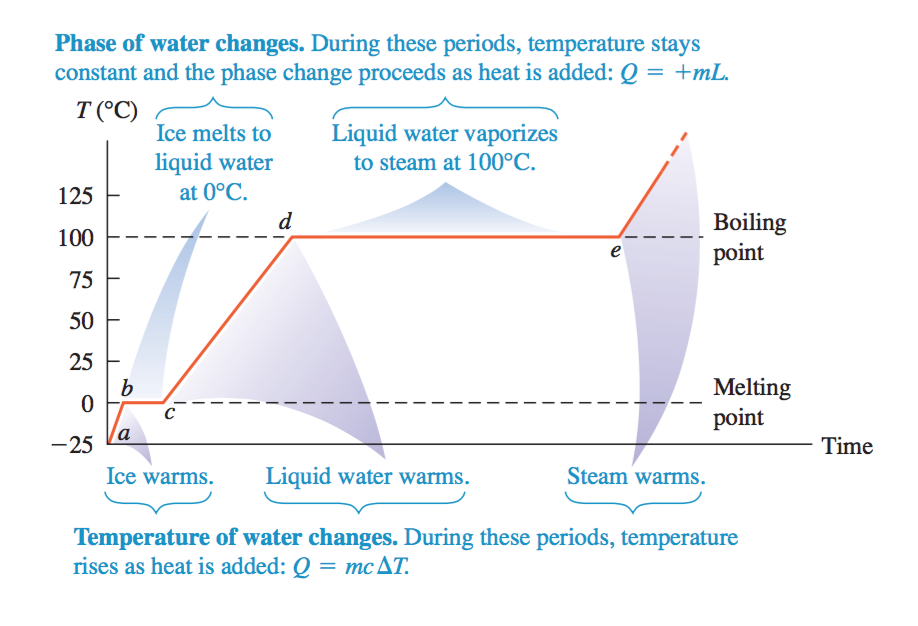
\includegraphics[scale=0.5]{data/img/plot}
	\caption{Cambios de fase del agua, según variaciones de la temperatura y del tiempo. Imagen tomada de \cite{young2011sears}, [Sears and Zemansky's, 2011]}
\end{figure}

Por último, la potencia puede medirse tomando la energía térmica sobre el sistema, por unidad de tiempo.

\section*{Procedimiento experimental}

Para medir el calor latente de fusión $L_f$ primero llenamos
el calorímetro con agua tibia (aproximadamente 40ºC) de masa $m_a$ , esperamos un minuto a que el agua y el calorímetro lleguen al equilibrio térmico, y medimos la temperatura inicial Ti. Añadimos hielo con masa $m_h$ y temperatura conocidas (el hielo debe dejarse unos minutos por fuera del congelador para que su temperatura sea de 0ºC y no menor), tapamos el calorímetro, esperamos a que se establezca el equilibrio térmico y medimos la temperatura de equilibrio $T_f$ .\\

\begin{figure}[htbp]
\centering
	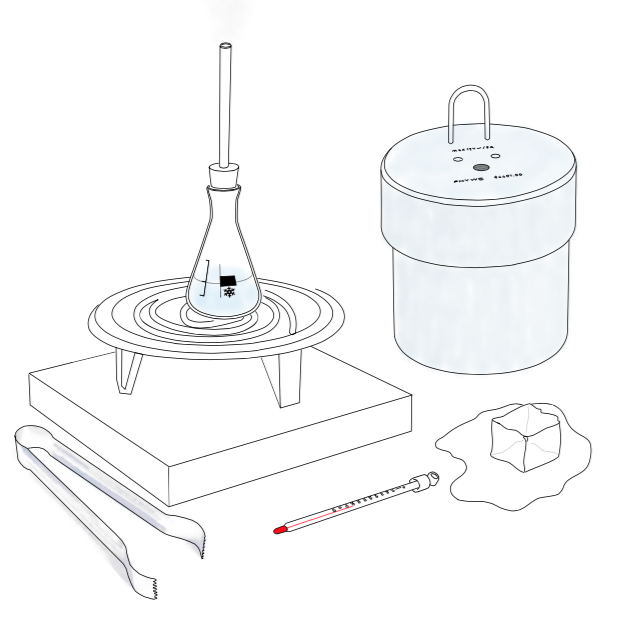
\includegraphics[scale=0.6]{data/img/proc}
	\caption{Disposición de materiales para la práctica, la imagen se encuentra en la guía de laboratorio}
\end{figure}

Para medir el calor latente de vaporizador primero determinamos la masa del matraz. Luego vertimos en el aproximadamente 70 mL de agua, determinando con la balanza la cantidad precisa. Prendemos la estufa, esperamos un minuto a que llegue a su temperatura de operación, ponemos el matraz sobre ella e iniciamos el cronometro. Determinamos la temperatura del agua a intervalos de un minuto. Cuando el agua comience a hervir retiramos con las pinzas y sumo cuidado el matraz de la estufa sin apagara, lo pesamos con ayuda de la balanza, y determinamos la masa de agua que llego hasta ese punto. Volvemos a poner, usan- do las pinzas, el matraz sobre la estufa, y cuando el agua comience a hervir iniciamos desde cero el cronometro y dejamos que la evaporación transcurra por un intervalo de tiempo $\Delta t$ tal que se evaporen mas o menos 5 mL de agua; retiramos de nuevo el matraz, pesamos con la balanza, determinamos el vapor de agua producido $\Delta m$ y volvemos a ponerlo sobre la estufa para que se evaporen mas o menos 5 mL adicionales; todos estos movimientos hechos con la mayor rapidez y cuidado posibles. Repetimos hasta que se hayan evaporado mas o menos 25 mL en total. Para reducir la variaron en la potencia transferida, procuramos poner el matraz siempre en el mismo punto de la estufa.
%----------------------------------------------------------------------------------------
%	REFERENCE LIST
%----------------------------------------------------------------------------------------

\begin{thebibliography}{99} % Bibliography - this is intentionally simple in this template

  \bibitem{young2011sears} Sears and Zemansky.B. {\em Sears and Zemansky's University Physics / Tutorials in Introductory Physics / Tutorials in Introductory Physics Homework. 17:565--567}, Pearson Education.  2011.
 
\end{thebibliography}

%----------------------------------------------------------------------------------------

\end{document}